\documentclass{article}
\usepackage[utf8]{inputenc}
\usepackage{graphicx}
\usepackage{enumerate}
\usepackage{amsmath}
\usepackage{amssymb}
\usepackage{amsthm}
\usepackage{verbatim}
\usepackage{float}
\usepackage{tikz}

\title{Testing the Kyle Lee Flow Market}
\author{Dan Friedman \and Yilin Li \and Kristian López Vargas}
\date{January 2021}

\begin{document}

\maketitle
\tableofcontents
\newpage

We will consider treatments with shredding bots in CDA and FBA.
Conjecture: do CDA or FBA with shredding bots approximate outcomes of the flow market?

We will define:

1) Environment

2) Treatment features. 

2.1) Formats KLFM (def CSLO), CDA, FBA

2.2) Strategy spaces: Bots / No bots. 
If bots, what can be tuned for the bots.
How the bots map bet parameters into order specs. 



%A 2018 term paper by Brett Williams and Sean Laney tries to shoehorn flow markets into the ELO environment. It convinced me (DF) that a different environment is needed for the Kyle-Lee flow (KLF) market to demonstrate its advantages and disadvantages relative to the usual stock market formats.

\section{Introduction}
Kyle and Lee (2017) developed the notion of an exchange that is fully continuous. We will refer to it as Kyle-Lee' Flow  Market (KLFM henceforth). In this market investors are able to shred orders more naturally, as part of the process to realign their portfolios. That is, an investor (maybe after reassessing an firm's prospects, or deciding to change her own goals, or perhaps due to an idiosyncratic shock in available funds to allocate) will place a bet of the form: by $t$ days (or perhaps minutes) from now, buy (or sell) $x$ shares at prices of up to (at least) $p$. 
To minimize price pressure, the investor will shred the shares orders. For example, they will do 50 transactions of size $\frac{x}{50}$, spread over time. Kyle thinks that flow orders will better enable investors to keep down transaction costs arising from price pressure.

In next draft, also explain here why KLFM may also help reduce inefficiencies associated with aggressive high frequency trade.

\section{Environment}
To capture those issues, let us define a new environment. The key idea is that investors treat the asset as having private value, as opposed to common value (assumed in many models and experiments in finance). We will refer to the new environment as KB (Kyle bets). % or as PV (private values).

We will discuss a simple version of this environment first, where bets are revealed privately at the same time and expire at the same time. Then we will discuss a more realistic environment where information and expiration are both random and asynchronous. 

\subsection{Static - Synchronous  }
The simplest version is static and synchronous in that the fundamental value V is constant, investors receive their private information simultaneously and share the same time horizon t.
Each investor $i$ (a human subject, or possibly a bot), receives a bet defined by the tuple $B_i = (x_i, p_i, \tau_i, t_i$). The elements of this tuple are interpreted as follows. At time $\tau_i$, investor $i$ is informed that at time $t_i$ $ (>\tau_i)$, the experimenter will privately place a limit order with her to buy up to $x_i$ units, if $x_i>0$, or will sell to her $|x_i|$ units, if  $x_i<0$, at price $p_i$. 

Initially we consider the static case, $\tau_i = 0$, and  $t_i = \bar{t}$, for all $i$. Which means, everyone receives their bet before the period starts and bets' expiration is shared by all investors.

The fundamental value $V$ is determined by equating the supply inherent in the $B_i$s with negative $x$ to the demand inherent in the bets with positive $x$.

\subsection{Dynamic - Asynchronous }
In the dynamic KB environment,  bets might arrive asynchronously after the trading period starts, and we allow for asynchronous horizons, $\tau_i \neq \tau_j$ and $t_i \neq t_j$ for $i\neq j$.

$V$ now is a function of $t$, and is determined as above by the set of all bets that have been received so far but have not yet expired. 


\section{Experiment Design}

Treatments will be defined in three dimensions:

\begin{enumerate}
    \item Market formats (CDA, KLFM, FBA)
    \item Strategies available (manual trading, algorithms with shredding, algorithms without shredding, etc)
    \item Market conditions (normal conditions, stressed/turbulent conditions)
\end{enumerate}

\subsection{Market Formats and Strategies}

\subsubsection{Continuous Double Auction (CDA)}
% \subsubsection*{Basic Rules}
% [Yilin bring rules from Aldrich LopezVargas]
The continuous double auction (CDA), also known as the continuous limit order book, works as follows. There is a \textit{limit order book} that sorts limit orders by (1) price and (2) time received (at each price). Bids are sorted from highest to lowest price and asks are sorted from lowest to highest price. The highest bid and the lowest ask are referred to as the \textit{best bid} and \textit{best ask}, respectively, and the difference between them is called the \textit{spread}.

Traders (whether human or automated) enter, replace, modify and cancel orders at any moment they choose and the CDA processes each limit order as it arrives. If the limit price locks (equals) or crosses (is beyond) the best contra-side price (e.g., if a new bid arrives with limit price equal to or higher than the current best ask) then the limit order immediately transacts at that best contra-side price, and the transacted quantity is removed from the order book. We say that limit order has been "executed" or "filled".  
On the other hand, if the price is no better than the current best same-side price, then the new order is added to the order book, behind other orders at the same price. That is at the same price and type of order, there is a queue where earlier orders have priority.
% The exchange breaks ties by randomly ordering messages received at the same price and time. Time priority in the CDA favors traders that can send, modify and cancel limit orders quickly, which results in all traders acquiring fast communication technology in the equilibrium.


\subsubsection{Kyle-Lee Flow Market}

% \subsubsection*{Basic Rules}

% \subsubsection*{Continuous Scaled Limit Orders (CSLO)}
Let us first define the \textbf{\textit{continuous scaled limit orders}, CSLO,} henceforth. The CSLO are messages with five parameters: a buy-sell indicator, a quantity $Q_{\max}$, two price levels $P_L$ and $P_H$ (with $P_L < P_H$), and the maximum trading speed $U_{\max}$. Such an order conveys the message, ``Buy up to a cumulative total of $Q_{\max}$ (shares) at maximum rate $U_{\max}$ (shares per hour) at prices between $P_L$ and $P_H$ (dollars per share)." The trading speed or flow demand $U(p(t))$ is a function of the market clearing price $p(t)$ given by 

$$U(p(t)) = \begin{cases}
	U_{max} & \text{if } p(t) < P_L \\
	\frac{P_H - p(t)}{P_H - P_L} U_{max} & \text{if } P_L \leq p(t) \leq P_H \\
	0 & \text{if } p(t) > P_H
\end{cases}$$

Similarly, the flow supply $U(p(t))$ is also a function of the market clearing price $p(t)$ given by 

$$U(p(t)) = \begin{cases}
	U_{max} & \text{if } p(t) > P_H\\
	\frac{p(t) - P_L}{P_H - P_L} U_{max} & \text{if } P_L \leq p(t) \leq P_H \\
	0 & \text{if } p(t) < P_L 
\end{cases}$$

If the price is strictly below (above) $P_L$ ($P_H$), the trader buys (sells) at the rate $U_{\max}$. If the price is strictly above (below) $P_H$ ($P_L$), the trader trades zero shares. If the price is between $P_L$ and $P_H$, the demand (supply) schedule is interpolated linearly, making its slope $\frac{(P_H - P_L)}{U_{\max}}$. \\

The cumulative quantity executed by time $t$ is 

$$Q(t_0,t) = \int_{t_0}^{t_0+t} U(p(\tau)) d\tau$$




\subsubsection{Frequent Batch Auction (FBA)}

% \subsubsection*{Basic Rules}

% [Yilin bring rules from Aldrich LopezVargas]

In a Frequent Batch Auction (FBA), the trading day is divided into submission stages of equal length $\tau$. These submission stages are referred to as \textit{batching intervals}. Within a batch interval, traders communicate with the exchange in continuous, sealed-bid fashion in order to privately submit, modify and cancel limit orders, which are collected and held by the FBA matching engine.

At the conclusion of a batch, all new orders are combined with unfilled orders from previous batches and the matching engine generates stair-step demand and supply curves from the aggregated bids and offers, respectively. If demand and supply do not intersect, no trade occurs and all orders carry over to the next batch, aside from those flagged as \textit{immediate} or \textit{cancel}. If demand and supply intersect, the market clears where supply equals demand, i.e., all infra-marginal bids and offers are executed at a uniform price $p^*$ that clears the market. The FBA matching engine then publicly broadcasts information regarding executed trades, $p^*$, and the remaining order book.


\subsection{Strategies and Algorithms}

\begin{enumerate}
    \item No Shredding Algo: Trade is analog. Human investors, if necessary, will shred orders by hand. 
    \item Shredding Algo: Trade can be automated and the algorithms can have a shredding option. To discuss: do we want to incorporate some kind of cost? If so what kind? fixed cost (building the algo), flow cost using the algo, fees for excessive messaging, etc.
\end{enumerate}

DF remark--shredding algos for CDA should include discrete approximations of a CSLO.

In KLFM, it remains unclear whether we should also deploy shredding algorithms. One option is investors can simply submit a continuous scaled limit order tailored to B and no option with algorithms. However, we can argue that using shredding algos might make the comparability with CDA stronger. 


\subsection{Market Conditions}

For the dynamic environment, we can deploy different market conditions as implemented in Aldrich and Lopez Vargas (e.g., higher or lower speed of change fundamental); or in ELOs current design with market thinning and or crashes. 

In the static environment, we can only vary the the thinness/thickness of the market, and the slopes of supply and demand as in classic CDA experiments. 

\subsection{Payoff functions}
At the end of a period, how do we calculate profits in a KB environment? 

To develop an answer, let's start with a standard indivisible unit induced value/cost environment for a CDA. Suppose that an agent has induced values $\{v_i\}_{i=1, ...,n}$ and/or induced opportunity costs 
$\{c_j\}_{j=1, ...,m}$. The convention is that $v_1 \geq v_2 \geq ... \geq v_n \geq 0$ and that $v_k=0$ for $k>n$. On the cost side, there is some upper bound $\bar{c}$ larger than any $v$ of any agent, such that $c_k=\bar{c}$ for $k>m$.
Again we make the convention that costs are sorted from most to least attractive: $0 \leq c_1 \leq c_2 \leq ... \leq c_m \leq \bar{c}$.

Suppose that our agent buys single units at prices $p_1, ..., p_N$ and sells single units at prices $r_1, ..., r_M$. 
Then her payoff is
\begin{align} \nonumber
    \pi = & [redemption payment - expenditure] + [revenue - opp. cost]  \\ \label{stairstepProfit}
    = & \sum_{i=1}^N [v_i - p_i]  + \sum_{j=1}^M [r_j - c_j]. 
 \end{align}

Dan thinks we can extend this idea to get what we want. The first extension is to allow for variable quantities, not necessarily single units, i.e., piecewise constant per-unit values and costs. The formula in (\ref{stairstepProfit}) needs to have appropriate $q_i$ and $q_j$ multiplying each term in each sum. 

The second extension is to have different 
redemption times for bets. I think it would work to apply the (q-modified) formula 
at each redemption time, and carry over positive or negative inventory and cash balances, after redeemed units (bought or sold to the experimenter) are removed.
Any carry over of positive inventory at the end of the period is valued at zero, and any negative inventory is backfilled at unit cost $\bar{c}$.

Fortunately, the price in each market institution, even KLFM, is piecewise constant as a function of time, so we can use sums as in (\ref{stairstepProfit}), rather than time integrals.

Kristian asks:
What is the advantage and disadvantage with respect to to setting a dynamic cap to buys equal to the trader's total active buy bets. And, similarly, a cap for sell orders equals the total active sell bets.
DF reply: I'd regard this as a last resort
in case lots of traders find themselves stuck at the end of the period (after the last bets are collected) with non-zero inventory.
Some traders might want to speculate 
earlier in the period and/or make markets, and imposing such a cap would interfere with that.

Yilin asks how we should think about opportunity costs $c_j$.
It is typical in lab experiments for many decades to induce supply in effect by offering a unit sell bet --- the human trader can sell a unit and keep the proceeds, but must reimburse the experimenter $c_j$ for it. If the trader doesn't sell the unit, there are no payoff consequences.
If she does sell at price $p$, her profit is
$p-c_j$; this will be negative when 
$p>c_j$. In that sense, the opportunity cost is $c_j$.

Yilin also asks about inducing both values and costs. I see no problem with that as long as $\min_i v_i > \max_j c_j$ at any given time; we don't want to earn arbitrage profits
via self-trading.

\subsubsection*{New Payoff}

Notation 
\begin{itemize}
    \item $Inv = inventory$
\end{itemize}



Assumptions

Endowment (initial cash) is zero.


% \begin{align*}
%     \Pi_t = \text{Locked In Profit}(t) 
% \end{align*}

\vspace{.2in}

\textbf{Intuition regarding profit display.} % Locked-in Profit Component.} 

The idea here is to display on the user interface an up-to-the-second summary of how well the trader has done so far (at time $t$) 
in taking advantage of her current bets (aka contracts).
The display will show locked-in profit as well as trading profit. Their sum is profit so far, and at the end of the period that sum is their profits for that period.

Conceptually, locked-in profit consists of the payoff the player would receive when the bet expires and they sell to (or buy from) the experimenter, if no more trades occur in the meantime. 
It must be disentangled from trading profitcode , i.e., profits from units already resold to (or repurchased from) other traders in the market. 
A disentangling
 requires some arbitrary conventions on which units  purchased count for the bet, and which units are retraded. 
Much of the complexity of the algorithm lies in consistently implementing those conventions.
A key step is to sort units by price paid, rather than by time acquired.

For example, suppose that a trader has a buy bet still active, and has bought two units at different prices and different times, and now sells a unit. If that unit is taken to be the more expensive of the two units in their inventory (as we shall implement below), then often the trading profit will be smaller but the  locked-in profit  larger than if we had used a different  convention, e.g., that the unit just sold was the first unit purchased.

To lay out the algorithm, let us begin with
a buy bet with given price, quantity and deadline  $(P_b,Q_b,T_b)$:

If $Inv_t>0$ and $Inv_t \leq Q_b$ then:\\
define $InvVecP_t = (p_1,p_2,p_3,..,p_{Inv_t}) $
where $p_{1,t}$ is the lowest price among the items in the current inventory, $p_2$ second lowest, and so on. This is the vector of sorted prices for a buy bet.
For that case define
    
    $$\text{Locked In Profit}(t) = 
    Inv \times P_b - \sum_{k=1}^{k=Inv} p_k$$
    
    $\text{Trading Profit} = $

    
If $Inv_t > Q_b$:

    $$\text{Locked In Profit}(t) = 
    Q_b \times P_b - \sum_{k=1}^{k=Q_b} p_k$$

That is, locked in profit is the sum of prices to be received when bet expires minus prices already paid for items sold, assuming that the trader always sells  the least expensive items of the current inventory to the experimenter when the bet expires.

Suppose there is a sell bet with price, quantity and deadline as in $(P_s,Q_s,T_s)$:

If $Inv_t < 0$ and $Inv_t \geq Q_s$:

    Let us define $InvVecP_t = (p_1,p_2,p_3,..,p_{Inv_t}) $
    Where $p_{1,t}$ is the highest price among the items in the current inventory, $p_2$ second highest, and so on. 
    
    $$\text{Locked In Profit}(t) = 
    Inv \times P_s - \sum_{k=1}^{k=Inv} p_k$$
    
If $Inv_t<Q_b$:

    $$\text{Locked In Profit}(t) = 
    Q_s \times P_s - \sum_{k=1}^{k=Q_s} p_k$$


    
    
% Inv * [Price_{\text{Buy Bet}} - \text{Average of Inv most cheapest items bought (from the start of the new bet? / or excluding items sold to previous bets)}]
	
Example: 

Buy Bet: Q=10, Price=12,
\begin{itemize}
    \item Buy 5 units at prices 8, 8, 10, 10, 10 \\
    Profit: 2 * (12 - 8) + 3 * (12 - 10) %
    \item Sell 2 units at 13 \\
    We are left with items at prices 8, 8, 10 \\
    Profit: 2 * (12 - 8) + 1 * (12 - 10)
    \item Buy two at 10 \\
    We are left with items at prices 8, 8, 10, 10, 10 \\
    Profit: 3 * (12 - 8) + 2 * (12 - 10) % 
\end{itemize}
DF thinks there is a typo in the very last expression.

May be express as the sum over the appropriate items.

Example

Bet is P=20; Q=10 \\
Inv = 4 \\
Bought 8 units  ( bought 4 at price 15, and 4 at price 18) \\
Sold 4 units at price 22 \\

Trading:  $(22-18) \times 4$ \\
Locked-in: $(20-15) \times 4$ \\

\subsubsection*{Recursive Formula}
\begin{itemize}
    \item Denote a trader's inventory at time $t$ as $Inv(t)$ \\
    $Inv(t) > 0$ means the trader has more units bought than units sold \\
    $Inv(t) < 0$ means the trader has more units sold than units bought  
    \item $s(\cdot)$ is a sorting function that sorts $\cdot$ by the sign of $Inv(t)$ 
    \item $InvVecP(t) = (p_1, p_2, p_3, ..., p_{Inv(t)})$ is a sorted vector of length $|Inv(t)|$ at any time $t$. \\
    It sorts $p_k$'s from low to high when $Inv(t) > 0$, while it sorts $p_k$'s from high to low when $Inv(t) < 0$
    \item $InvVecP(t) = (p_1, p_2, p_3, ..., p_{Inv(t)})$ \\
    where 
    \begin{align*}
        p_1 < p_2 < ... < p_{Inv(t)}, & \text{ when } Inv(t) > 0\\
        p_1 > p_2 > ... > p_{Inv(t)}, & \text{ when } Inv(t) < 0
    \end{align*} 
    \item Assume a \textbf{buy bet} is represented with price, quantity and deadline as in $(P_b, Q_b, T_b)$ ($P_b > 0$, $Q_b > 0$)
    \item Denote $\min\{\max \{Inv(t), 0\}, Q_b\}$ as $\underline{Q}$
    % $\max 0 and \min\{Inv(t), Q_b\}$ as $\underline{Q}$
    \item Assume a \textbf{sell bet} is represented with price, quantity and deadline as in $(P_s, Q_s, T_s)$ ($Q_s < 0, P_s > 0$) 
    \item Denote $\max\{\min \{Inv(t), 0\}, Q_s\}$ as $\overline{Q}$
\end{itemize}

\noindent 
\textbf{Buy Bet} 

\begin{itemize}
    \item bet starts
    \begin{itemize}
        \item $InvVecP(t) = InvVecP(t^-)$
        \item $Inv(t) = Inv(t^-)$
        \item $cash(t) = cash(t^-)$
        \item $\text{locked-in profits}(t) = 
        \begin{cases} 
            0, & Inv(t) \leq 0 \\
            \underline{Q} \times P_b - \sum^{k = \underline{Q}}_{k = 1} p_k, & Inv(t) > 0 
        \end{cases}$
    \end{itemize}
    \item bet ends
    \begin{itemize}
        \item $InvVecP(t) = 
        \begin{cases}
            InvVecP(t^-), & Inv(t) \leq 0 \\
            s(InvVecP(t^-) \setminus \{p_k\}_{k = 1}^{k = \underline{Q}}, & Inv(t) > 0 
        \end{cases}$
        \item $Inv(t) = 
        \begin{cases}
            Inv(t^-), & Inv(t) \leq 0 \\
            Inv(t^-) - \underline{Q}, & Inv(t) > 0
        \end{cases}$
        \item $cash(t) = cash(t^-) + P_b \times \underline{Q}$
        \item $\text{locked-in profits}(t) = 0$
    \end{itemize}
    \item buy 1 unit at price $p$ \\
    For flow market, record the prices for each fractional share of a single unit and update the locked-in profit when each single unit bought or sold. \\
    For example, suppose a trader bought 0.3 unit at price 100, another 0.3 unit at price 100, and another 0.5 unit at 110, then the price $p$ for this 1 unit bought is the weighted average of all fractional prices, $0.3 \times 100 + 0.3 \times 100 + 0.4 \times 110 = 104$. The leftover 0.1 unit remains. 
    \begin{itemize}
        \item $InvVecP(t) = 
            \begin{cases}
                s(InvVecP(t^-) \cup \{p\}), & Inv(t^-) \geq 0 \\
                s(InvVecP(t^-) \setminus \{p_{Inv(t)}\}), & Inv(t^-) < 0    %%% recover the cheapest unit sold previously 
            \end{cases}$
        \item $Inv(t) = Inv(t^-) + 1$
        \item $cash(t) = cash(t^-) - p$
        \item $\text{locked-in profits}(t) = 
        \begin{cases} 
            \text{locked-in profits}(t^-) + (P_b - p),  & 0 \leq Inv(t^-) < Q_b \\
            \text{locked-in profits}(t^-) + (p_{Q_b} - p), & Inv(t^-) \geq Q_b, p < p_{Q_b} \\
            \text{locked-in profits}(t^-), & \text{otherwise}
        \end{cases}$
    \end{itemize}
    \item sell 1 unit at price $p$ \\ %that was bought at $p_{Inv(t)}$ \\  %%% sell the most expensive unit first \\
    For flow market, record the prices for each fractional share of a single unit and update the locked-in profit when each single unit bought or sold. \\
    For example, suppose a trader sold 0.4 unit at price 100, another 0.3 unit at price 100, and another 0.3 unit at 110, then the price $p$ for this 1 unit sold is the weighted average of all fractional prices, $0.4 \times 100 + 0.3 \times 100 + 0.3 \times 110 = 103$. 
    \begin{itemize}
        \item $InvVecP(t) = 
        \begin{cases}
            s(InvVecP(t^-) \setminus \{p_{Inv(t)}\}), & Inv(t) > 0 \\
            s(InvVecP(t^-) \cup \{p\}), & Inv(t) \leq 0
        \end{cases}$
        \item $Inv(t) = Inv(t^-) - 1 $
        \item $cash(t) = cash(t^-) + p$
        \item $\text{locked-in profits}(t) = 
            \begin{cases} 
            \text{locked-in profits}(t^-) - (P_b - p_{Inv(t)}), & 0 < Inv(t^-) \leq Q_b \\
            \text{locked-in profits}(t^-), & \text{otherwise}
            \end{cases}$
    \end{itemize}
\end{itemize}

\textbf{Sell Bet} \\

\begin{itemize}
    \item bet starts
    \begin{itemize}
        \item $InvVecP(t) = InvVecP(t^-)$
        \item $Inv(t) = Inv(t^-)$
        \item $cash(t) = cash(t^-)$
        \item $\text{locked-in profits}(t) = 
        \begin{cases} 
            \sum^{k = |\overline{Q}|}_{k = 1} p_k - |\overline{Q}| \times P_s, & Inv(t) < 0 \\
            0, & Inv(t) \geq 0 
        \end{cases}$
    \end{itemize}
    \item bet ends
    \begin{itemize}
        \item $InvVecP(t) = 
        \begin{cases}
            s(InvVecP(t^-) \setminus \{p_k\}_{k = 1}^{k = |\overline{Q}|}), & Inv(t) < 0 \\
            s(InvVecP(t^-), & Inv(t) \geq 0
        \end{cases}$
        \item $Inv(t) = 
        \begin{cases}
            Inv(t^-) + |\overline{Q}|, & Inv(t) < 0 \\
            Inv(t^-), Inv(t) \geq 0
        \end{cases}$
        \item $cash(t) = cash(t^-) + P_s \times \overline{Q}$
        \item $\text{locked-in profits}(t) = 0$
    \end{itemize}
    \item buy 1 unit at price $p$ %that was sold at $p_{Inv(t)}$
    \begin{itemize}
        \item $InvVecP(t) =
            \begin{cases}
                s(InvVecP(t^-) \setminus \{p_{Inv(t-)}\}), & Inv(t^-) < 0 \\
                s(InvVecP(t^-) \cup \{p\}), & Inv(t^-) \geq 0
            \end{cases}$
        \item $Inv(t)= Inv(t^-) + 1$
        \item $cash(t) = cash(t^-) - p$
        \item $\text{locked-in profits}(t) = 
        \begin{cases} 
            \text{locked-in profits}(t^-) - (p_{Inv(t^-)} - P_s),  & Q_s \leq Inv(t^-) \leq 0, \\  %%% recover the cheapest unit sold previously 
            \text{locked-in profits}(t^-), & \text{otherwise}
        \end{cases}$
    \end{itemize}
    \item sell 1 unit at price $p$ 
    \begin{itemize}
        \item $InvVecP(t) =
                 \begin{cases}
                     s(InvVecP(t^-) \cup \{p\}), & Inv(t^-) \leq 0 \\
                     s(InvVecP(t^-) \setminus \{p_{Inv(t^-)}\}), & Inv(t^-) > 0
                 \end{cases}$
        \item $Inv(t) = Inv(t^-) - 1$
        \item $cash(t) = cash(t^-) + p$
        \item $\text{locked-in profits}(t) = 
        \begin{cases} 
            \text{locked-in profits}(t^-) + (p - P_s),  & Q_s < Inv(t^-) \leq 0 \\
            \text{locked-in profits}(t^-) + (p - p_{Q_s}), & Inv(t^-) \leq Q_s \text{ and } p > p_{Q_s} \\
            \text{locked-in profits}(t^-), & \text{otherwise} 
        \end{cases}$
    \end{itemize}
\end{itemize}

\section{Alternative Profit Signal}
$$\text{projected cash}(t) = \begin{cases}
    cash(t) + P_B \times \min\{\max\{0, Inv(t)\}, Q_B\}, & \text{Buy bet} \\
    cash(t) - P_S \times \min\{-Inv(t), Q_S\}, & \text{Sell bet} \\
    cash(t) - P_m \times (-Inv(t) - Q_S), & \text{Sell bet, and } -Inv(t) > Q_S
\end{cases}$$

\section{Things to discuss and decide}
\begin{itemize}
    \item So we want speed tech available?  
    \item How can we display bets and trading profits?
\end{itemize}
Regarding the second item, I think we can build a unified display of locked in and potential profits, that can also display live bets. This is what I have in mind.
\begin{itemize}
\item live bet(s). A bet is displayed as a rectangle of height P and width Q in the positive orthant. The entire rectangle is shaded light gray if the player has not yet made any transactions. 
\item For concreteness in the following description, I assume a buy bet: at time T=121, the experimenter will pay the player P=11 per unit for up to Q=20 units. Sell bets are analogous...
\item As the player purchases units (via accumulating flows in KLF or in discrete chunks in CDA or FBA), the units acquired are sorted from lowest purchase price to highest, and displayed inside in the same graph as the bet. \item This will create a piecewise constant increasing schedule that looks like a supply curve. Call it $S(t).$ It lies above the horizontal axis between 0 and $q(t)$, the accumulated quantity purchased so far. 
\item For $q(t)<Q,$ and $t<T$, color the area [between $S(t)$ and the horizontal line at $P=11$, from 0 to $q(t)$] green where $S(t)<11=P$ and red where $S(t)>11=P$, but keep it gray beyond $q(t).$ Profit locked in so far is the green area minus the red area.
\item At $t=T$, flash the red and green areas, show their numerical values, and book the net profit in an appropriate box. Remove the $P \times Q$ rectangle.
\item If $q(T)>Q,$ then slide the residual over to the vertical axis. That is, for $t$ slightly larger than $T$, $q(t) = q(T)-Q,$ and $S(t)$ is the segment that used to be beyond the bet box.
\item If there is no active bet, we can show trading profits in a similar fashion.
\item Purchases so far are still shown as an expenditure area below a supply/cost curve S, sorted by increasing price up to cumulative quantity purchased, just as above. 
\item Sales so far are shown as a revenue area below a demand/value curve, sorted by decreasing price up to cumulative quantity sold. 
    \item The area between S and D is shaded green (indicating positive profit) where $D>S$ and is shaded red (indicating negative profit) where $D<S$. 
\item When cumulative quantity purchased differs from cumulative quantity sold, extend the shorter curve at 0 if D, and at $\bar{c}$ if S, until curves extend to the max cumulative quantity.
\item Update this graph dynamically as transactions flow.
\end{itemize}
% Yilinhttps://www.overleaf.com/project/6011fe74c7d0656d63338d48
% This makes very much sense to me. different color-shaded areas will make it easier for subjects to understand what is going on with legends indicating what each color represents
% I think it is helpful if we can distinguish transactions with traders and with the experimenter 

Comment. \\
We may want to use slightly different color codes for $D$ or $S$ that comes from a bet (induced by the experimenter) from the portion of all over $D$ or $S$ that comes from accumulated actual transactions. The bet $D$ or $S$ is guaranteed but has not yet actually taken place.

\section{Coding Inputs (temporary)}

\subsection*{Parameterization of environment}

\begin{itemize}

    \item Frequency of update $\delta$: \\
    FLO 20ms \\
    CDA 20ms \\
    FBA (max batch length 5000ms) 

    \item $P_{\min}$ / $P_{\max}$: \\
    FLO $P_{\min} \leq P_{\max}$ \\
    CDA $P_{\min} = P_{\max}$ \\
    FBA $P_{\min} = P_{\max}$ 

    \item Max rate of execution $U_{\max}$ (per second):  \\
    FLO $U_{\max} \in (0, 1,000,000]$ \\
    CDA $U_{\max} = 1,000,000$ \\ 
    FBA $U_{\max} = 1,000,000$ 
    
\end{itemize}

%%%%%%%%%%%%%%
\newpage
\appendix

\section{Appendix - Theory}

\subsection{Kyle Lee Flow Market}

\noindent
Suppose the aggregate demand and supply schedules intersect at a point where either of the two is not flat. Then the excess demand schedule $D(p) - S(p)$ is strictly decreasing in the neighborhood of the intersection. The exists a ``best bid" price $P_B$ and ``best ask" price $P_A$, both on the tick grid, where $P_A$ is one tick size large than $P_B$, and there is excess demand at the best bid and excess supply at the best ask price given by 

$$D(P_B) - S(P_B) > 0 \quad \text{ and } \quad S(P_A) - D(P_A) > 0$$

\noindent
Define the relative order imbalance $\omega \in [0,1]$ by 

$$\omega = \frac{D(P_B) - S(P_B)}{D(P_B) - S(P_B) + S(P_A) - D(P_A)}$$

\noindent
Then the market clearing price $p(t)$ is uniquely defined by 

$$p(t) = P_B + \omega (P_A - P_B)$$

\noindent
Intuitively, the price is a weighted average of the two prices $P_B$ and $P_A$, with weights $1-\omega$ and $\omega$ proportional to the excess demand and supply at these prices. 

\begin{figure}[H]
\centering
\caption{Continuous Scaled Limit Order Book}
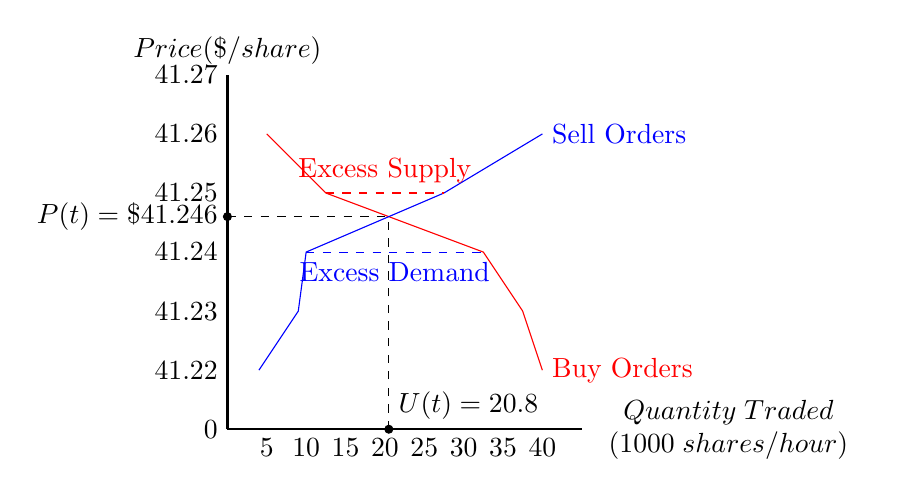
\begin{tikzpicture}[scale=0.5]
\draw[thick,-] (0,0) -- (0,9) node[above]{$Price (\$/share)$};
\draw[thick,-] (0,0)--(9,0) node[right]{\begin{tabular}{c}
     $Quantity \; Traded$ \\
     $(1000 \; shares/hour)$
\end{tabular}};
\node[left] at (0,1.5) {$41.22$};
\node[left] at (0,3.0) {$41.23$};
\node[left] at (0,4.5) {$41.24$};
\node[left] at (0,6.0) {$41.25$};
\node[left] at (0,7.5) {$41.26$};
\node[left] at (0,9.0) {$41.27$};
\node[below] at (1,0) {$5$};
\node[below] at (2,0) {$10$};
\node[below] at (3,0) {$15$};
\node[below] at (4,0) {$20$};
\node[below] at (5,0) {$25$};
\node[below] at (6,0) {$30$};
\node[below] at (7,0) {$35$};
\node[below] at (8,0) {$40$};
\node[left] at (0,0) {$0$};
\draw[red,solid] (1,7.5) -- (2.5,6.0) -- (6.5,4.5) -- (7.5,3) -- (8,1.5) node[right]{Buy Orders} ;
\draw[blue,solid] (0.8,1.5) -- (1.8,3) -- (2,4.5) -- (5.5,6) -- (8,7.5) node[right]{Sell Orders};
\draw[red,dashed] (2.5,6.0) -- (5.5,6.0);
\draw[blue,dashed] (2,4.5) -- (6.5,4.5);
\node[red,above] at (4,6.0) {Excess Supply};
\node[blue,below] at (4.25,4.5) {Excess Demand};
\draw[dashed] (4.1,0) -- (4.1,5.4);
\draw[dashed] (0,5.4) -- (4.1,5.4);
\node[above right] at (4.1,0) {$U(t)=20.8$};
\draw[fill] (4.1,0) circle [radius=.1];
\node[left] at (0,5.4) {$P(t)=\$41.246$};
\draw[fill] (0,5.4) circle [radius=.1];
\end{tikzpicture}
\end{figure}

\noindent
Figure 2 depicts the market clearing with continuous scaled limit orders. Both the downward sloping supply schedule and the upward sloping demand schedule are piece-wise linear functions of price with knot points at which prices are integer multiples of the minimum tick size of \$0.01 and quantities are integer multiples of one share per hour. The unique price, \$41.246 per share, is not an integer multiple of minimum tick size. The unique quantity, 20800 shares per hour, happens to be an integer number of shares per hour. Each supply and demand schedule will flow their U(\$41.246) shares per hour at the price \$41.246.



%%% Instructions

\section*{Experiment Instructions (Flow Market)}

Welcome, and thank you for participating!

\noindent
From now until the end of the experiment, please do not communicate with other participants. If you have any questions, please raise your hand; an experimenter will come and answer your question.

\noindent
Please pay careful attention to the instructions as real money is at stake.
During the experiment you will earn Experimental Currency Units (ECUs) and at the end of the experiment all your earnings will be converted to US dollars at the rate of one dollar for every two ECUs. You are guaranteed a show up fee of \$X.00 but can earn considerably more. 

\subsection*{Basic Ideas} 
In this experiment, you will participate in a simple \textbf{automated financial market}. Using information displayed on your screen as in Figure 1, you will \textbf{set and adjust trading strategies} so as to earn as many ECUs as you can. As explained below, your earnings will depend on the settings you choose and on the choices of \textbf{the other XX participants} in your group. There will be \textbf{XX trading periods}, each lasting \textbf{four minutes}, after which the experiment will end and you will be paid. 

%%%%%%%%%% Figure 1 of UI %%%%%%%%%%
\textbf{\large Insert a screenshot of UI?  }

\noindent
\textit{\textbf{Buy Orders and Sell Orders.}} All participants submit buy
orders and sell orders. The orders consist of five elements: a buy/sell indicator, the maximum cumulative total of shares to trade, the low price of the order, the high price of the order, and the maximum rate of shares to trade per unit of time. Submitting a buy order for up to a cumulative of 50 shares at maximum rate 500 shares per hour at prices between 90 and 110, for example, means that you are willing to pay 110 ECUs or less to buy up to 50 shares of the stock at maximum rate of 500 shares per hour.
Similarly, if you submit a sell order for up to a cumulative of 50 shares at maximum rate 500 shares per hour at prices between 90 and 110, you are willing to receive 90 ECUs or more to sell a share of the stock at maximum rate of 500 shares per hour.

\noindent
\textit{\textbf{Experimenter Bet.}} At random times an experimenter bet arrives at participants to buy X shares of the stock at price XX at time TT or to sell X shares of the stock at price XX at time TT. An experimenter bet that says ``Buy 10 shares at price 100 ECUs per share at time 3:30" means that the experimenter will buy up to 10 shares of the stock from you to help offset your positive inventory at price 100 ECUs per share at time 3:30. Similarly, an experimenter bet that says ``Sell 15 shares at price 100 ECUs per share at time 2:30" means that the experimenter will sell up to 15 shares of the stock to you to help cover your negative inventory at price 100 ECUs per share at time 2:30.


\subsection*{Your Choices and Earnings}

\noindent
\textit{\textbf{Trader.}} As a trader, you can post both a buy order and a sell order using the computer program (henceforth, ``your bot") shown in XXXXX. These orders are represented by ........... To adjust your orders, simply drag the XXX in the plot to indicate the low price, high price, and the maximum rate of your order and input the maximum cumulative quantity in the box. You can cancel you old orders and send new orders at anytime within each trading period. 

\noindent
You make a profit when other participants buy shares from you at higher prices than your original costs of purchasing them. Otherwise, you may also make a profit if you buy shares at lower prices than the price from the experimenter's buy bet or if you sell shares at higher prices than the price from the experimenter's sell bet. Your profits from transactions with other participants are accrued immediately in your cash account whereas your profits from experimenter bet are denoted as \textbf{locked-in profits} and will be added to your cash account until the bet's deadline passes. 

\noindent
You can also lose money (earn a negative profit). For example, suppose you have a buy bet but you bought shares of the stock at prices greater than the price offered in the bet, then you will incur a loss as the cost of buying those shares is higher than the revenue from selling them. Similarly, you will lose money if you sold shares of the stock at prices lower than the price listed in the bet when you have a sell bet. 

\noindent
\textit{\textbf{Session Earnings.}} Your final earnings for the session will be the sum of your show up fee and the profits of one randomly chosen trading period, converted into US dollars. 



\end{document}

% Tue 8 Nov 2022
% Discuss stability

